\documentclass{beamer}
\usetheme{Madrid} % clean, professional theme
\usepackage[utf8]{inputenc}
\usepackage{amsmath,amssymb}
\usepackage{graphicx}

\title{Cavity Flow: Numerical Simulation}
\author{Masud}
\date{\today}

\begin{document}

% Title slide
\begin{frame}
\titlepage
\end{frame}

% Outline slide
\begin{frame}{Outline}
\tableofcontents
\end{frame}

% Introduction
\section{Introduction}
\begin{frame}{Cavity Flow Problem}
The lid-driven cavity flow is a classical CFD benchmark for incompressible Navier-Stokes equations.

\[
\begin{aligned}
\frac{\partial \mathbf{u}}{\partial t} + (\mathbf{u} \cdot \nabla) \mathbf{u} &= - \nabla p + \nu \nabla^2 \mathbf{u}, \\
\nabla \cdot \mathbf{u} &= 0
\end{aligned}
\]

\begin{itemize}
    \item $\mathbf{u} = (u,v)$ is the velocity vector
    \item $p$ is pressure
    \item $\nu$ is kinematic viscosity
    \item Top lid moves with constant velocity; other walls are stationary
\end{itemize}
\end{frame}

% Numerical Method
\section{Numerical Method}
\begin{frame}{Discretization}
\begin{itemize}
    \item Uniform Cartesian grid: $x_i, y_j$
    \item Time-stepping: explicit or semi-implicit schemes
    \item Finite difference / finite volume approximations:
    \[
    \frac{u_i^{n+1}-u_i^n}{\Delta t} + u_i^n \frac{u_{i+1}^n - u_{i-1}^n}{2 \Delta x} + v_j^n \frac{u_{j+1}^n - u_{j-1}^n}{2 \Delta y} = -\frac{\partial p}{\partial x} + \nu \nabla^2 u
    \]
    \item Pressure correction via SIMPLE or PISO algorithm
\end{itemize}
\end{frame}

% Boundary Conditions
\begin{frame}{Boundary Conditions}
\begin{itemize}
    \item Top lid: $u = U_{lid}, \quad v = 0$
    \item Side and bottom walls: $u = v = 0$ (no-slip)
    \item Pressure: $\partial p/\partial n = 0$ at walls
\end{itemize}
\end{frame}

% Example
\section{Example}
\begin{frame}{Simulation Results}
\begin{figure}[h]
\centering
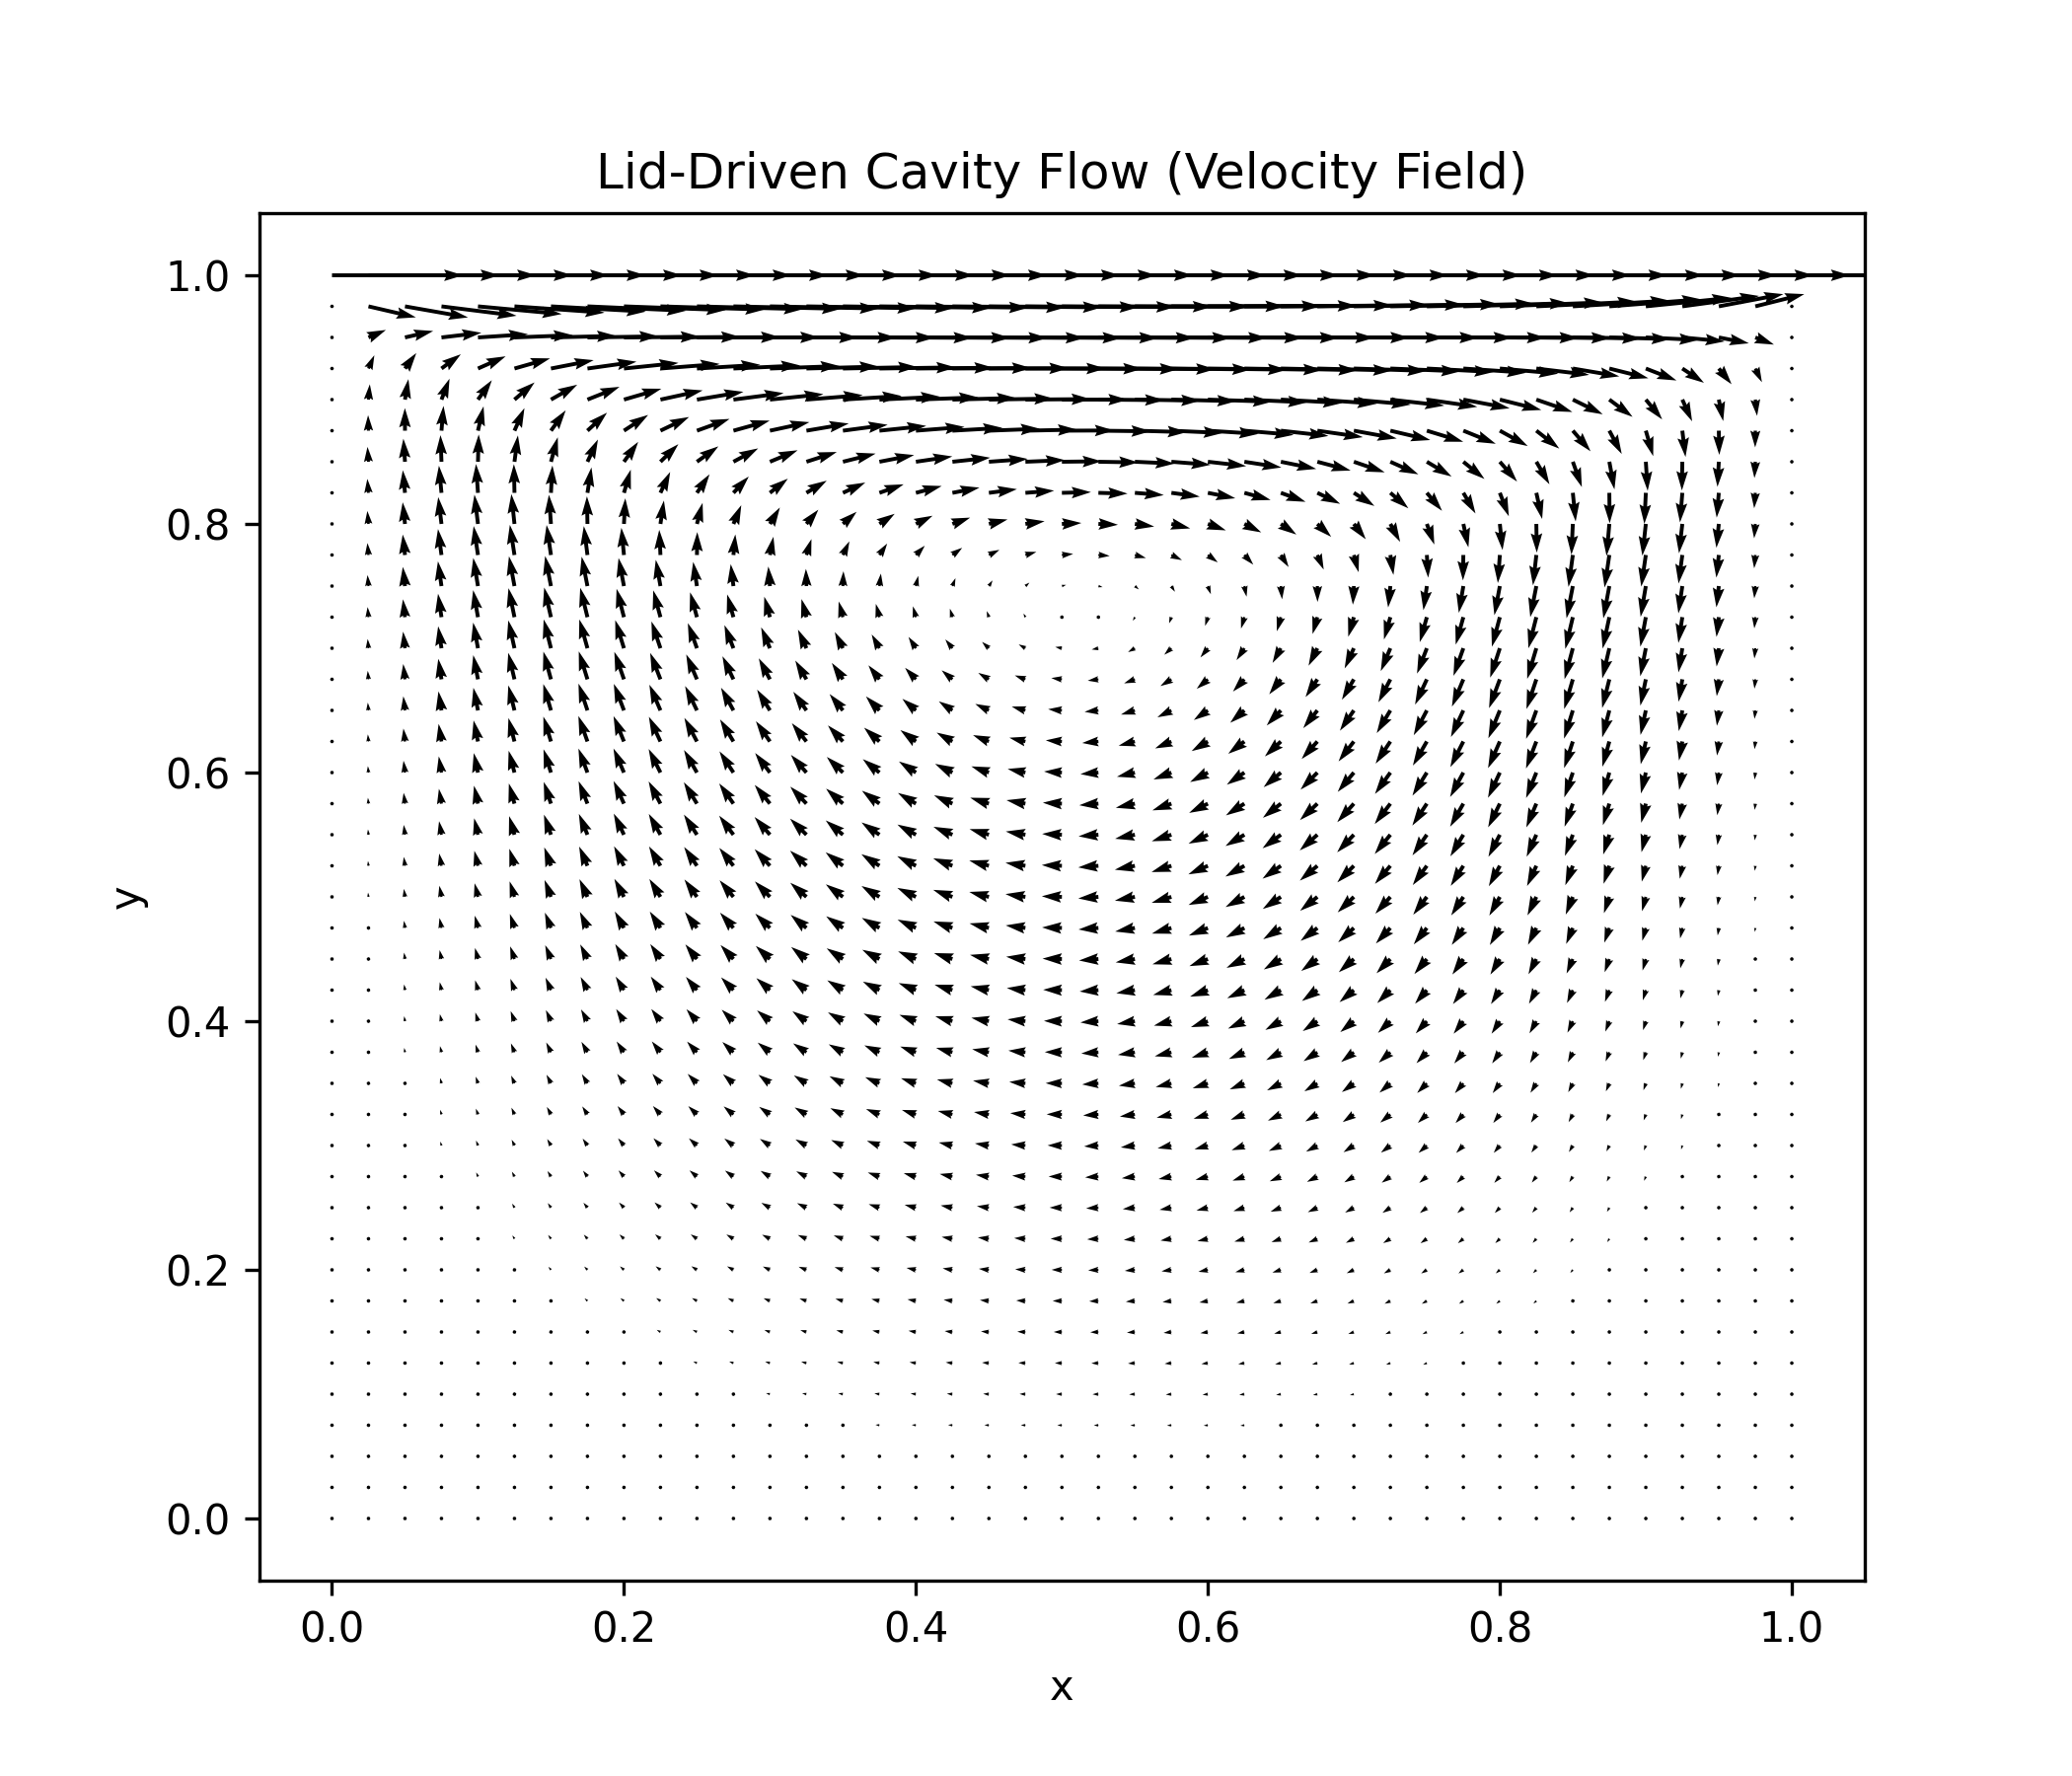
\includegraphics[width=0.8\linewidth]{cavity_flow.png} % replace with your figure
\caption{Velocity field in a square cavity (numerical solution)}
\end{figure}
\end{frame}

% Discussion
\section{Discussion}
\begin{frame}{Observations}
\begin{itemize}
    \item Formation of primary vortex in cavity center
    \item Secondary corner vortices appear at higher Reynolds numbers
    \item Steady-state solution obtained after sufficient time steps
    \item Benchmark for testing CFD solvers and pressure-correction algorithms
\end{itemize}
\end{frame}

% Conclusion
\section{Conclusion}
\begin{frame}{Conclusion}
\begin{itemize}
    \item Lid-driven cavity flow is a standard CFD benchmark problem
    \item Numerical solution demonstrates incompressible flow behavior and vortex formation
    \item Useful for validating CFD methods like SIMPLE, PISO, or FVM solvers
\end{itemize}
\end{frame}

\end{document}
